% Poster-native rubric bar chart. Wider bars, tighter category spacing,
% legend out of the bar area, taller y-axis labels.
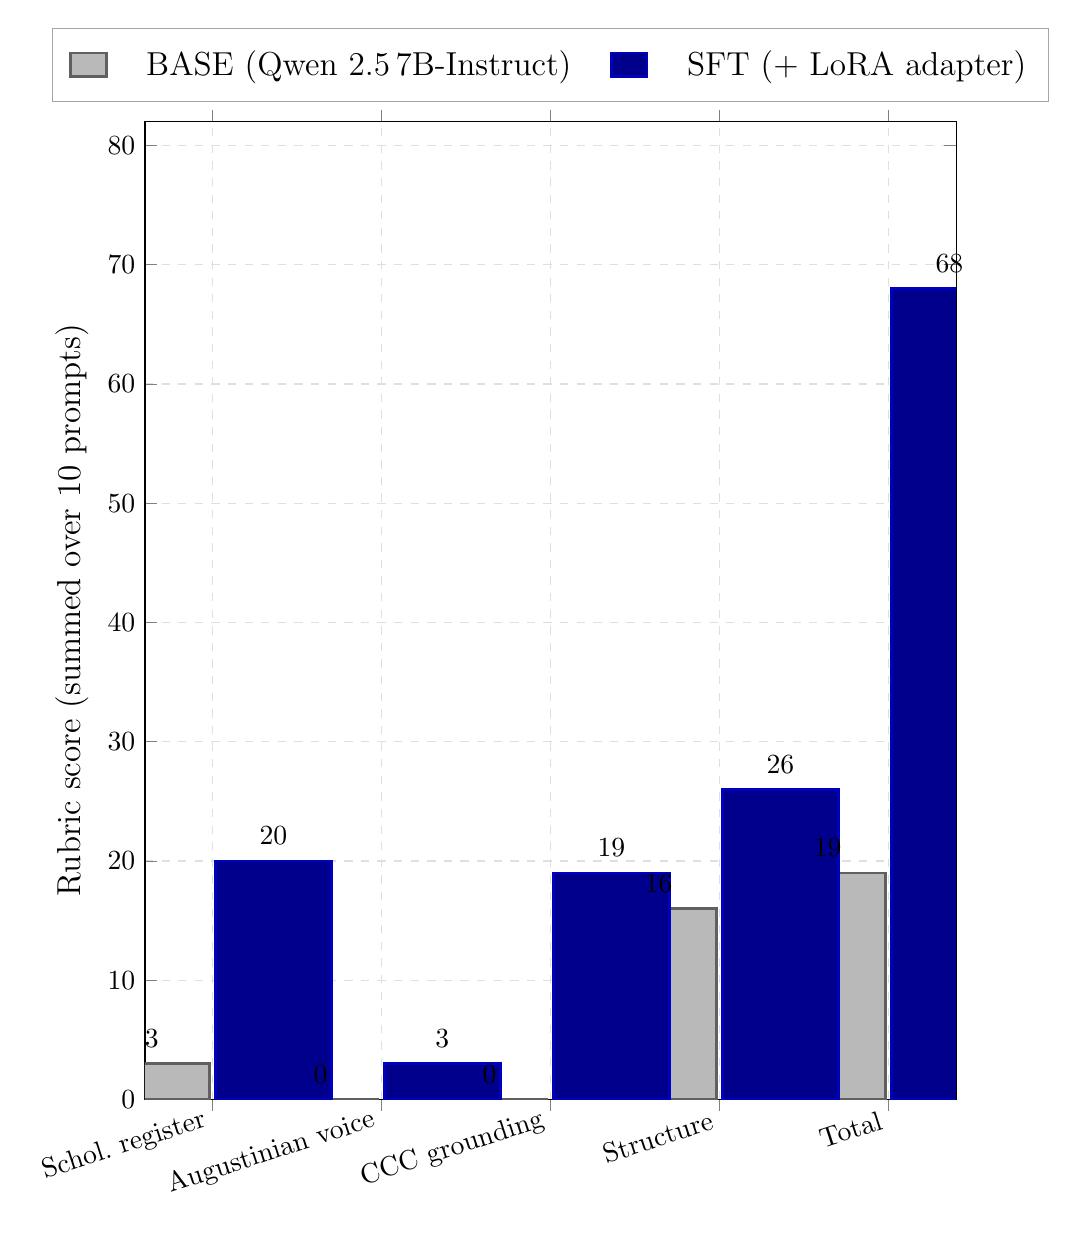
\begin{tikzpicture}
\begin{axis}[
    width=0.98\linewidth,
    height=14cm,
    ybar,
    bar width=42pt,
    ymin=0, ymax=82,
    enlarge x limits=0.10,
    ylabel={Rubric score (summed over 10 prompts)},
    symbolic x coords={Schol.\ register, Augustinian\ voice, CCC\ grounding, Structure, Total},
    xtick=data,
    x tick label style={font=\normalsize, rotate=18, anchor=east, yshift=-2pt},
    y tick label style={font=\normalsize},
    ylabel style={font=\large},
    nodes near coords,
    nodes near coords style={font=\normalsize, anchor=south, yshift=2pt},
    legend image code/.code={
      \draw [#1] (0cm,-0.15cm) rectangle (0.45cm,0.15cm);
    },
    legend style={
      at={(0.5,1.02)},
      anchor=south,
      legend columns=-1,
      font=\large,
      fill=white,
      draw=black!35,
      column sep=1.2em,
      inner sep=6pt,
    },
    grid=major,
    grid style={dashed,gray!25},
    every axis plot/.append style={line width=1pt},
  ]

  \addplot[fill=gray!55, draw=gray!75!black] coordinates {
    (Schol.\ register, 3)
    (Augustinian\ voice, 0)
    (CCC\ grounding, 0)
    (Structure, 16)
    (Total, 19)
  };
  \addlegendentry{BASE (Qwen 2.5\,7B-Instruct)}

  \addplot[fill=blue!55!black, draw=blue!75!black] coordinates {
    (Schol.\ register, 20)
    (Augustinian\ voice, 3)
    (CCC\ grounding, 19)
    (Structure, 26)
    (Total, 68)
  };
  \addlegendentry{SFT (+ LoRA adapter)}

\end{axis}
\end{tikzpicture}
